
\documentclass{article}
\usepackage[a4paper, total={6in, 8in}]{geometry}


\usepackage[utf8]{inputenc} % Unicode source support
\usepackage{graphicx} % Required for inserting images
\usepackage{amsmath}
\usepackage{amsthm}
\usepackage{float}
\usepackage{tikz}
%\usepackage{apalike}
\usepackage{amssymb}
\usepackage{amsfonts}
\usepackage{multicol}


\theoremstyle{definition}
\newtheorem{definition}{Definition}[section]

%\usepackage[backend=biber,style=apa]{biblatex}

%, citestyle=apa, sorting=ynt
\usepackage[colorlinks=true,citecolor=black, urlcolor=blue
]{hyperref}
\usepackage{verbatim}

\usepackage{url}
\def\UrlBreaks{\do\/\do-} % NIIIIICEEEE AAAA
\DeclareMathOperator{\so}{SO}
\DeclareMathOperator{\divergence}{div}
\DeclareMathOperator{\lensop}{L}
\newcommand*{\lens}[2]{\lensop\left(#1,#2\right)} %
% \DeclareUnicodeCharacter{2254}{\coloneq} % ≔
\renewcommand{\S}{\mathbb{S}}
\newcommand{\Z}{\mathbb{Z}}


%\usepackage[hyphens]{url}
%\usepackage{natbib}
\usepackage{dirtytalk}
\usepackage{mathtools}

\title{
{\leavevmode \smash {
\includegraphics[scale=0.4]{rug_logo.png}}}\\
    \vspace{1cm}
{Computing CMB temperature fluctuations for spherical
spaces} \\\ Preparation Bachelor's Project}

\author{Javier Gustavo Vela Castro \footnote{\href{mailto:j.g.vela.castro@student.rug.nl}{j.g.vela.castro@student.rug.nl
}}, Adriel Matei \footnote{\href{mailto:a.r.matei@student.rug.nl}{a.r.matei@student.rug.nl}}
, Juš Kocutar\footnote{\href{mailto:j.kocutar@student.rug.nl}{j.kocutar@student.rug.nl}}, Béla Schneider \footnote{\href{mailto:b.g.schneider@student.rug.nl}{b.g.schneider@student.rug.nl
}}}

\date{28th February 2025}


\begin{document}
\maketitle


\section{Abstract}

We present a study of cosmic microwave background (CMB) temperature fluctuations in spherical spaces, which are the models of the universe where the space is a 3-dimensional sphere or its quotient. We give an overview of the preliminary machinery used in the study of CMB temperature fluctuations for spherical space. We examine the behavior of isospectral but not isometric spherical forms. We explore the problem of testing for anisotropies in the mean of CMB temperature fluctuations for spherical spaces.

\section{Introduction}
The cosmic microwave background (CMB) is the electromagnetic radiation left from the Big Bang.  Temperature fluctuations provide an idea of the early state of the universe, as well as possible hints on its current shape. Observations of space missions such as COBE, WMAP and PLANK have revealed an unexpectedly low variance in CMB anisotropies, which are small variations in the radiation, at really large angular scales \cite{aurich_2012}. This goes against the expected results of the infinite and flat universe from the standard $\Lambda$CDM model.

This motivates exploring cosmological models beyond the infinite flat spaces. One possible explanation is that the universe is not infinite, as often assumed, but finite and multiconnected, the latter means it is connected but not simply connected. Specifically, if we consider the universe to be a finite spherical space (positively curved and closed, rather than infinite and flat), this would naturally introduce an upper limit to the size of CMB fluctuations \cite{aurich_2012}, potentially explaining lower large-angle correlations. 

The spherical space topology has been studied as a candidate for the shape of the universe by many researchers. For example, the 3-sphere $\mathbb{S}^3$ and its quotient manifolds can produce lower CMB power on large scales due to their finite size \cite{aurich_2012}. Some authors systematically examined entire families of spherical topologies such as lens spaces $L(p,q) = \mathbb{S}^3/Z_p$ (taking the quotient of $\mathbb{S}^3$ by the group of rotations of order $p$) with $p\le 500$ being the upper bound \cite{aurich_2012}. While such models did not show a dramatically strong suppression of CMB power in the tested range, they set an important methodology for how one might analyze and compare CMB temperature  fluctuations in spherical space models. The important component of the articles involved is how these theoretical results compare to observations and what do they imply about the possible (shape) topology of the universe.


\section{Preliminaries}
\subsection{Manifolds}
Metric and topological spaces allow us to generalize concepts from analysis like limits, sequences, and continuity. As a reminder, metric spaces generalize distance and topological spaces generalize open sets, which can both be used to redefine all these other concepts from analysis. This is useful, as it allows those concepts to be used in completely different settings.

The definition of a topological space is too general to meaningfully describe physical reality. The concept of topological manifolds tries to limit the potential pathological examples of topological spaces by requiring the spaces to look Euclidean at a local level. Formally, this means that any point on the set has a neighborhood around it equivalent (homeomorphic) to an open set of Euclidean space.

\begin{figure}[h]
    \centering
    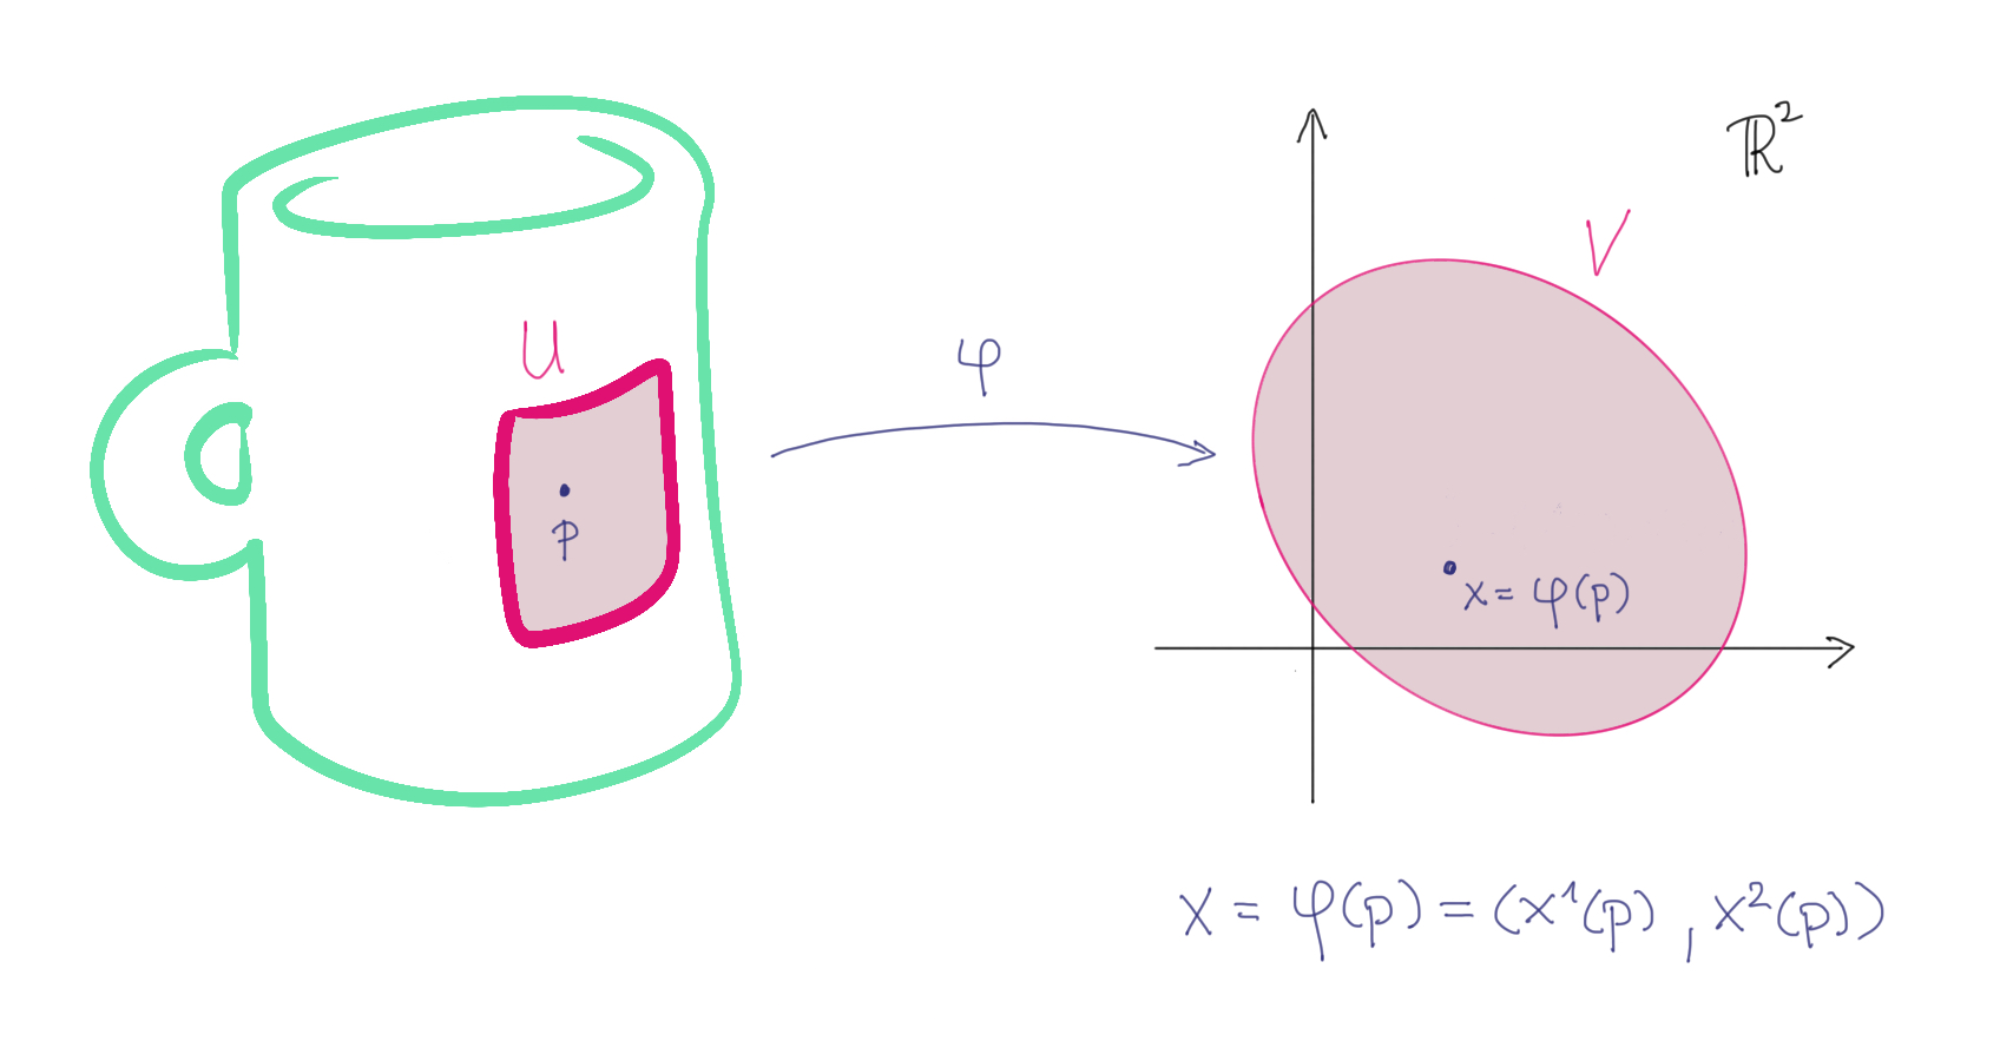
\includegraphics[width=0.5\linewidth]{mug-neighbourhoods.png}
    \caption{The prototypical example of a manifold -- a mug. Image source: \cite{serri}}
    \label{fig:mug-neighbourhoods}
\end{figure}

\begin{definition}
    A topological space $M$ is a \textbf{topological manifold} of dimension $n$, or topological $n$-manifold, if it has the following properties: 
    \begin{itemize}
        \item $M$ is a Hausdorff space,
        \item $M$ is second countable,
        \item $M$ is locally euclidean of dimension $n$, that is, for any point $p \in M$ there exist an open subset $U \subset M$ with $p \in U$, and open subset $V \subset \mathbb{R}^n$ and a homeomorphism $\varphi: U \rightarrow V$.
    \end{itemize}
\end{definition}

Where second-countability is defined as follows.

\begin{definition}[]
    A topological space $(X,T)$ is said to be \textbf{second countable} if there exists a countable set $B \subset T$ such that any open set can be written as a union of sets from $B$. In such case, $B$ is called a (countable) basis for the topology $T$ .
\end{definition}

%This is very useful, as it allows us to `pull back' many familiar concepts from Euclidean space (for instance, derivatives). Still, this turns out not to be enough. Analysis is built upon limits and sequences, yet those building blocks can behave in unexpected ways when taken out of the Euclidean setting.

For one, limits need not be unique in the general case. This could happen if there are not enough neighborhoods to direct the sequence to a single point, which is why we require manifolds to be Hausdorff.


Moreover, sequences are just functions from the naturals to our space, so they are inherently `countable' in nature. Indeed, we are used to many nice properties of limits. For instance, if a function in real space preserves the limits of sequences, then it is guaranteed to be continuous. But such a test might not hold in the general case. Indeed, there could be too many neighborhoods around each point, such that a simple sequence does not suffice for detecting properties like continuity. Requiring the space to be first countable (that is, requiring that each point has a countable basis for its neighborhoods) solves this issue. In fact, we require an even stronger condition for manifolds in second countability (that is, a countable basis must exist for the entire space). %%I'm actually not super sure what second countability adds over first countability here, but perhaps even first countability can have the issue of ``too many open sets'' (this time at a global level). 


For a more in-depth treatment of manifolds and their manifold properties, the reader should consider \cite{serri}. A more thorough exposition of the way limits and sequences break down in the general setting (and how we can work around that) can be found in the third chapter of \cite{topcat}.

When transporting (i.e. moving) a vector around a loop on a flat plane, the vector will arrive at the starting point in the same orientation it left as. This turns out not to be the case in the more general setting. We can quantify the amount by which this fails around every point using the concept of Gaussian curvature. Intuitively, when the curvature is $0$, the space is flat (at a point). When the curvature is positive, the space is convex (around said point), giving rise to spherical geometry. Otherwise, the space is hyperbolic (around the point). For larger dimensions, the Riemann curvature tensor allows us to take the Gaussian curvature along different slices formed by different sections.

A natural application of the above is detecting the curvature of the universe itself, i.e. the nature of the (spatial) geometry in which we exist. Our best tool when it comes to trying to detect such matters is the study of the cosmic microwave background radiation. In particular, this article is interested in the consequences of assuming that the underlying geometry is spherical. Indeed, although this might sound trivial (i.e. the universe would spatially be the surface of a giant four-dimensional ball), more interesting spaces arise when we allow the underlying space to have `holes'.

Topologically, holes can be detected using homology groups (the abelian group of loops in the space, under the identification of loops that can be smoothly transformed into each other as equivalent). In particular, a space is contractible if any loop can be smoothly transformed into the trivial loop (a path that never leaves the initial point). That is, the (first) homology group must be trivial. We say a space is simply connected when it is both contractible and path connected (i.e. every two points are connected by a path). 

\begin{figure}[H]
    \centering
    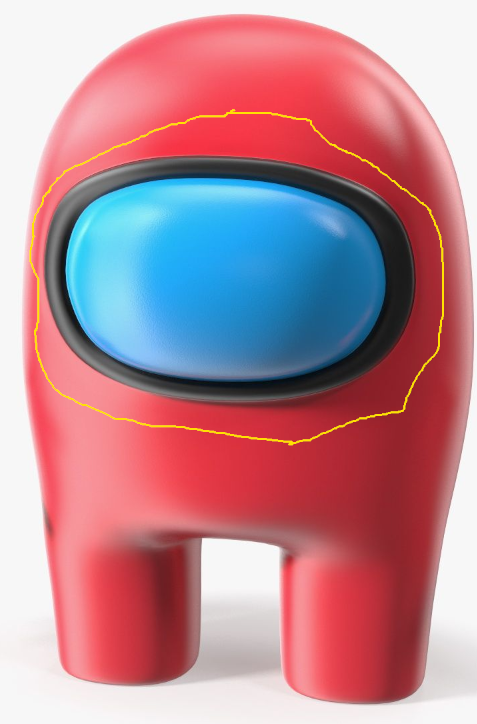
\includegraphics[width=0.25\linewidth]{amogus.png}
    \caption{The yellow path is non contractible on the space highlighted in red (there's an additional hole in the back of the figure, thus the path cannot simply contract through there)}
    \label{fig:amogus}
\end{figure}


In what follows we use the concrete definition of the 3-sphere as an embedded submanifold of $\mathbb{R}^4$ lying in Euclidean space meaning $\mathbb{S}^3 := \{x \in \mathbb{R}^4 \; |\; \|x\| = 1\}.$ Next we define a certain special set of matrices which induce well-defined maps on the sphere.

\begin{definition}
    We define $$SO(4) = \{A \in \mathbb{R}^{4 \times 4}:\; A^TA = I_4, \; \det(A) = 1\}.$$
\end{definition}

By the standard action of $\mathbb{R}^{4 \times 4} $ on $\mathbb{R}^4$ we have that $SO(4)$ is naturally a subgroup of the group of isometries of $\mathbb{S}^3$. This is because for any $x \in \mathbb{S}^3$ we get $$\|Ax\| = (Ax)^T(Ax) = 
x^T(A^TA)x = x^Tx = \|x\| =1$$
hence $Ax \in \mathbb{S}^3$ implying $A|_{\mathbb{S}^3}$ is a well-defined map and a bijection. By analogous reasoning, we find that:

$$\|Ax - Ay\| = \|A(x-y)\| = \|x-y\|,$$ hence $A$ is an isometry.

Now, for any subgroup $H \leq SO(4)$ we can consider the orbits of the action of $H$ on $\mathbb{S}^3$. We recall from group theory that this produces an equivalence relation on $\mathbb{S}^3$ where $x \sim y$ whenever $x$ and $y$ are in the same orbit of $H$. That is, the set of equivalency classes of $\mathbb S^3$ with 
$$x \sim y \,\iff\, \exists\, g\in H: x = g\cdot y.$$ 

The set $\mathbb{S}^3/_\sim$ can be given a manifold structure if certain conditions on the projection $\pi: \mathbb{S}^3 \to\mathbb{S}^3 /_\sim $ are satisfied, the details can be found in \cite{serri}. For instance, if $H$ is a finite subgroup of $SO(4)$ then the manifold $\mathbb{S}^3 /_\sim$ is a 3-manifold which has positive curvature, similar to $\mathbb{S}^3$.

\begin{comment}

There is an alternative way of viewing the quotient $\mathbb{S}^3/\Gamma$ using the concept of a covering space.  In particular for our universe, the spaces are interested in are quotients $\mathbb S^3 /_\sim$ for various groups $\Gamma$ of covering transformations (i.e. transformations that shuffle around the different copies of the underlying manifold which tile the covering space). 

\begin{definition}[Covering spaces]
    A covering space $\tilde X$ for a space $X$ is a (continuous) map $\pi : \tilde X \to X$, such that every point $x \in X$ has a neighborhood $U_x$ such that $\pi ^{-1} (U_x) = \coprod_{d \in D_x} V_d$ for some indexing set $D_x$ and sets $V_d$ such that $\pi |_{V_x} : V_x \to U_x$ is a homeomorphism.
\end{definition}

\begin{figure}[h]
    \centering
    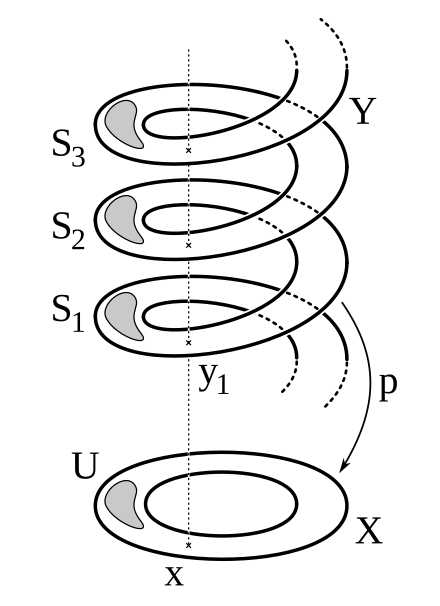
\includegraphics[width=0.25\linewidth]{covering-space.png}
    \caption{The space $Y \coloneq [0, 1] \times \mathbb R$ is a covering space for $X \coloneq [0,1] \times \S^1$. The disjoint open sets $S_i$ are mapped homeomorphically onto $U$. The fiber of $x$ consists of the points $y_i$. Source: \cite{wiki:covering} }
    \label{fig:enter-label}
\end{figure}
\end{comment}

 


\section{Discussion of results from selected articles}

\subsection{The spectral geometry of hyperbolic and spherical spaces (E. A. Lauret and B. Linowitz)}

In \cite{emilio}, the authors go over the theoretical grounding of the literature on the topic. The candidate manifolds for the shape of the universe are, as discussed above, manifolds of the form $\mathbb S^3 / \Gamma$ (for some subgroup $\Gamma$ of the isometry group of the sphere, i.e. $\so(4)$). We will refer to such spaces as `space forms.

An important class of manifolds are the so-called `lens spaces', which correspond to the case where $\Gamma$ is cyclic and the dimension of the underlying manifold is odd. As we are interested in studying the shape of our (spatially) three-dimensional universe, all the spaces we are interested in will be lens spaces as long as $\Gamma$ is cyclic. 

\begin{definition}[Lens spaces]
    Formally, we denote by $\lens q s$ (where $q \in \mathbb N$, $s \in \mathbb Z ^n $ and $\gcd(q, s_i) = 1$ for all $i$), the space $\mathbb S^{2n - 1} / \Gamma _{q;s}$, where $\Gamma_{q;s}$ is the (cyclic) group generated by the diagonal matrix with diagonal entries $R(2 \pi s_i/ q)$ (where $R(-)$ is a two-dimensional rotation matrix by the given angle).
\end{definition}
The condition $\gcd(q, s_i) = 1$ is necessary to ensure that $\Gamma$ acts freely on $\mathbb S^{2n-1}$.

The Laplace-Beltrami operator generalizes the Laplace operator on smooth functions defined on $\mathbb{R}^n$ to general manifolds. 
\begin{definition}[Laplace-Beltrami operator]
  The Laplace-Beltrami operator is defined as the divergence of the gradient:
  \begin{align*}
      \Delta f \coloneqq \divergence (\nabla f)
  \end{align*}
\end{definition}

In particular, the spectrum of Laphlace-Beltrami operator (collection of eigenvalues) in $L^2(M, g)$ is a discrete subset of the non-negative reals, in which every value occurs with a finite multiplicity. Two such manifolds are said to be isospectral if they share a spectrum. 


Inverse spectral geometry studies the different ways in which the spectrum affects different properties of the underlying space. For instance, the dimension and volume of a manifold are completely determined by its spectrum. However, this spectrum does not completely determine the manifold uniquely up to isometry.

\subsubsection{Volume maximizing isospectral pairs of sphere forms}

The first important problem tackled by \cite{emilio} is that of determining the isospectral sphere form pair (that is, a pair of spaces that are isospectral yet not isometric) of largest volume. According to \cite{ikeda80}, if $\mathbb S^{2n-1}/\Gamma_1$ and $\mathbb S^{2n-1}/\Gamma_2$ are isospectral spherical forms, the two groups have equal order and equal set of element orders. As a consequence, one is cyclic only if the other is cyclic (thus one space is a lens space if and only if the other is as well). 

After classifying $\Gamma$ for spherical forms with homotopy group of order strictly smaller than $24$ and non-cyclic into four specific groups of different orders (the specific groups are irrelevant here), the paper concludes that if a pair of odd-dimensional isospectral but not isometric spherical space forms exists with fundamental group of order strictly less than $24$, then the two are cyclic (otherwise one of the two would be one of the four groups classified above, but then so would the other, as by \cite{ikeda80} isospectral pairs share their cyclic-ness), and thus lens spaces. The isospectral pair with the largest volume must then also be the one containing lens spaces (since no other kind of pair can exist for such groups). The paper then defines a way to generate larger lens spaces from smaller ones by concatenating the indices (which we denoted earlier by $s$, and can be treated like ordered lists here). Together with a computational search, the paper was able to build a table of the precise lens spaces that maximize volume for multiple dimensions, although whether lens spaces are the solutions for all dimensions is still an open question.


\subsubsection{The silver lining}

While the study of isospectral pairs is indeed interesting, we can take solace in knowing that no such pairs exist in dimension three. That is, for the purpose of this article, all pairs of isospectral sphere forms must also be isometric. The motivated reader is encouraged to read \cite{emilio} for further details.













\subsection{CMB Anisotropy of Spherical Spaces (R. Aurich, S. Lustig and F. Steiner)}




In \cite{aurich_2005} the authors consider the 3-manifolds of the form $\mathcal{M} := \mathbb{S}^3 /_ \sim$ where $\sim$ is an equivalence relation coming from identifying orbits of some finite subgroup of the special linear group $SO(4)$.

On any smooth manifold we can define the notion of smooth functions and the Laplace-Beltrami operator $\Delta$, as explained before. One can then consider the solutions of the so-called Helmholtz equation on $\mathcal{M}$ given by 

$$(\Delta + E_\beta^\mathcal{M})\psi_\beta^{\mathcal{M}, i} = 0$$
where $E_\beta^\mathcal{M} \in \mathbb{R}$ the functions $\psi_\beta^{\mathcal{M}}$ is a smooth function on $\mathcal{M}$ and $\beta \in \mathbb{N}.$ We call the function $\psi_\beta^\mathcal{M}$ the eigenmode of the Helmholtz operator and $E_\beta^\mathcal{M}$ the corresponding eigenvalue.
As explained in \cite{luminet_2005}, we can lift any eigenmode $\psi _\beta^\mathcal{M}$ of the Helmholtz equation on $\mathcal{M}$ to an $H$-invariant eigenmode
${\psi'}_\beta^\mathcal{M}$ on $\mathbb{S}^3$, meaning it satisfies the Helmholtz equation
and ${\psi'}_\beta^\mathcal{M}(hx) = {\psi'}_\beta^\mathcal{M}(x)$ for all $h \in H$.


From \cite{aurich_2005} we see that, in fact, the spectrum of the Helmholtz operator is a discrete subset of $\mathbb{R}$ and that $E_\beta = \beta^2 - 1$ for $\beta \in \mathbb{N}$, we call $\beta$ a wave number. However, depending on the group $H$, not all wave numbers $\beta$ are possible.


For instance, if $H = {1}$, the trivial group, we know that the set of wave numbers is $\mathbb{N}$ itself, i.e. no restrictions. If $H = Z_m$, i.e. the cyclic group where $m$ is an odd number we get that the set of wave numbers is  $\{1,3,\cdots, m\}\cup \{m+1, m+2, m+3, \cdots \}$.


Furthermore, we can then expand any eigenfucntion of the Helmholtz operator on $\mathcal{M}$ in terms of eigenfunctions on $\mathbb{S}^3$ which are explicitly known and the authors know how to compute the coefficients.

Section 3 of \cite{aurich_2005} forms the technical part of their paper. The complete understanding of it also requires a certain background in cosmology. Their goal is to compute the relative fluctuations $\frac{\delta T}{T}$ of CMB for all of the spherical manifolds obtained as the quotients of finite subgroups of $SO(4)$. First, they explain how the CMB fluctuations arise as manifestations of different effects such as the Sachs-Wolfe contribution. For the calculations they assume that the initial values for the fluctuations for each wave number were certain Gaussian random variables.


After the derivation they arrive, for each spherical manifold, the value for the angular power spectrum $\delta T^2_l$ for $l = 1,2,3$, which are certain real numbers which can be directly derived from $\delta T$ after writing


$$\delta T  (\hat{n}) =\sum_{l \geq 2}\sum_{m = -l}^{m = l}a_{lm}\tilde{Y}(n)$$

in terms of spherical harmonics $\tilde{Y}_{lm}$ which comprise an orthonormal basis for $L^2(\mathbb{S}^2)$ (the two sphere $\mathbb{S}^2$ is the natural domain for the CMB when we observe it.)

The definition of the angular power spectrum is then 

$$\delta T^2_l = \frac{l(l+1)}{2}\frac{1}{2l+1 }\left\langle \sum_{m = -l}^la_{lm}^2\right\rangle.$$



They plot, for each spherical manifold, $\delta T_l^2$ with respect to $\Omega_{tot}$. The variable $\Omega_{tot}$ is the density parameter of the universe, and can be obtained from measurements. In the same plot they also show $\delta T^2_l$ as measured in WMAP.

\subsection{Results}


The authors conclude that the spherical manifolds which align closest with the measured data are the ones obtained when setting $H = O^*$ and $H = I^*$, the binary octahedral and binary icosahedral group respectively, which are respectively of order 48 and 120. The authors presented an explicit description of the groups generated by left- and right- multiplication of certain quaternions, but we will not go in detail here.


Furthermore, they excluded other groups such as the binary tetrahedral group $T^*$ and infinite families of binary dihedral groups and cyclic groups as possible models because they exhibited drastically different behavior.
























\subsection{CMB radiation in an inhomogeneous spherical space}
In \cite{Aurich_2011}, the authors consider the CMB in spherical 3-manifolds that are inhomogeneous. Specifically, the space which we are working with is of the form $\mathbb S^3/\Gamma$, where $\Gamma$ is a group acting on $\mathbb S^3$ and the quotient is the set of orbits. 

%This can also be seen as a covering, where $\S^3$ is the covering space, $\S^3/\Gamma$ is the space being covered, $\Gamma$ is the automorphism group and $\pi: x\mapsto \Gamma x$ is the covering map. 
The condition of the manifold being inhomogeneous means that, unlike the 3-sphere $\mathbb S^3$ and 3-torus $\mathbb T^3$, the manifold does not look the same at each point on the manifold. Because of inhomogeneity, the CMB is very much dependent on the point of observation. 

In the article, the authors discuss different spherical 3-manifolds, classifying whether they are inhomogeneous, analyzing their properties, and finding equivalences. For example, some of the manifolds in question are the lens manifolds $L(p,q)$ and the cubic manifolds $N2$ and $N3$.

One important concept is the fundamental domain. Given our manifold $\mathbb S^3/\Gamma$, a fundamental domain is a subset of $\S^3$, which under the action of $\Gamma$ can reach the entirety of $\S^3$. Moreover, all non-identity elements of $\Gamma$ must send elements in this set outside of it. Intuitively, it is a set of representatives of $\S^3/\Gamma$ which are all next to one another, similarly to how $\Z/n\Z$ has $\{0,1,\dots,n-1\}$ as such a set. There is one specific fundamental domain that we care about, called the Voronoi domain. Given our observation point $x_0\in\S^3$, the Voronoi domain is the set of elements $x\in\S^3$ such that the following holds:

$$ d(x_0,x) \leq d(x_0,g\cdot x) \quad \forall\, g\in\Gamma $$

where $d(\cdot,\cdot)$ is the $\S^3$-distance.

To figure out whether a spherical manifold is homogeneous, one must understand what the group action does under a change of observer position. Changing the observer position is done mathematically by applying a change of coordinates $u'=uq$ with $u\in\S^3$ and the isometry $q\in\text{SU}(2,\mathbb C) \equiv \S^3$, making $u=q^{-1}$ the new origin $u'=q^{-1}q=e$. Now, using the general group element $g = (g_l,g_r)\in\Gamma$ and letting $\tilde u = g\cdot u = (g_l)^{-1}ug_r $, we get $ \tilde u' = (g_l)^{-1} u' (q^{-1}g_rq) $. This means that the transformation in our shifted space is $g' = (g_{l},q^{-1}g_{r}q)$, which is not the same as $g$ in general, so if $g_r = q^{-1}g_rq$ does not always hold in a manifold, it is inhomogeneous.

All of this can be used to figure out the observer-dependent CMB variations and other related values in different inhomogeneous spherical manifolds.



\subsection{Test for anisotropy in the mean of the CMB temperature fluctuation in spherical harmonic space}
The temperature fluctuations of the Cosmic Microwave Background (CMB) provide crucial insights into the physics of the early universe and the underlying cosmological model. 

From the point of view of Earth, we can view CMB as a function defined on the celestial sphere $\mathbb{S}^2$. Hence we can express CMB as the sum of spherical harmonics - a certain family of smooth functions defined on $\mathbb{S}^2$ which forms an orthonormal basis for $L^2(\mathbb{S}^2)$, meaning they are orthogonoal and of size 1, whith respect to the $L^2$ inner product.

Following the article by Kashino et al. (2012), this section goes through an overview of a mathematical method for computing and interpreting CMB temperature fluctuations in spherical spaces, incorporating statistical isotropy, covariance structures, and Monte Carlo simulations, which are later compared with the Wilkinson Microwave Anisotropy Probe (WMAP) seven-year observation data \cite{Kashino_2012}. \\
The observed temperature fluctuations along a given direction on the celestial sphere can be expanded using spherical harmonics
\[\Delta T(\hat{n}) = \sum_{\ell=0}^{\infty} \sum_{m=-\ell}^{\ell} a_{\ell m} Y_{\ell m}(\hat{n}),\]
where $\Delta T(\hat{n})$ are fluctuations on the CMB temperature field, $Y_{\ell m}$ are the spherical harmonic functions evaluated in the direction of $\hat{n}$, and $a_{\ell m}$ are the spherical harmonic coefficients encoding temperature fluctuations at different scales. \\
Under the assumption that the primordial fluctuations are statistically homogeneous and isotropic in the mean, and assuming they obey the Gaussian distribution, with the $2\ell+ 1$ spherical harmonic coefficients $a_{\ell m}$ for each $\ell$ being independent Gaussian variables, then the coefficients should satisfy the following condition:
\[\langle a_{\ell m} \rangle = 0, \quad \langle a_{\ell m} a^*_{\ell' m'} \rangle = C_\ell \delta_{\ell \ell'} \delta_{m m'}\]

Here $\langle ... \rangle$ denotes the average, $C_\ell$ is the ensemble average power spectrum, which describes the variance of temperature fluctuations as a function of angular scale and $\delta$ is the Kronecker symbol. \\
Thus, if the mean is nonzero $\langle a_{\ell m} \rangle \neq 0$, it \textbf{suggests possible anisotropies or preferred directions in the universe}. 

Since real CMB observations are affected by instrumental noise and sky masking, estimating $C_\ell$ accurately requires simulations. Given a theoretical power spectrum $C^{th}_\ell$, the corresponding harmonic coefficients are drawn from a Gaussian distribution:
\[
a_{\ell m} \sim \mathcal{N} (0, C_\ell^{\text{th}})
\]

Applying a sky mask function $M(\hat{n})$ modifies the observed coefficients:

\[
a^{\text{mask}}_{\ell m} = \sum_{\ell' m'} M_{\ell m, \ell' m'} a^{\text{all sky}}_{\ell' m'}
\]

where $a^{\text{all sky}}$ is taken from the all sky CMB map (which we can
never obtain), and $M_{\ell m, \ell' m'}$ is the convolution matrix of
the mask. This introduces mode coupling, which must be corrected using a decorrelation transformation based on the eigenvalue decomposition of the covariance matrix.

To test the assumption of statistical isotropy, we examine the mean of $a_{\ell m}$ across multipole bins. The test statistic is defined as:
\[
S_i = \sum_{j} W_{ij} M_j
\]
where $W$ is a decorrelation matrix derived from the covariance structure. If significant anomalies appear in the mean values of $a_{\ell m}$, this suggests deviations from isotropy that may indicate the need for new theories.

For plotting, we used the results of different frequency channels used in the CMB analysis, originating from the WMAP (Wilkinson Microwave Anisotropy Probe) data. This corresponds to the following frequency band categories: Q-band $(\~40 GHz)$, V-band $(~60 GHz)$ and W-band $(~90 GHz)$ \cite{Jarosik_2011}. Each band has slightly different noise levels and sensitivity to galactic foregrounds.

Taking these data, we plot the comparison between expected noise levels and observed anomalies in the mean multipole moments. Let the x-axis represent the multipole moment $\ell$, which corresponds to angular scales, with lower values representing large-scale features and higher values representing smaller-scale fluctuations. The y-axis represents the test statistic $S_i$, which quantifies deviations from statistical isotropy, or in other words the temperature fluctuations from the expected results for an isotropical space. 

The multipole moment $\ell$ and the angular scale $\theta$ are inversely related. The higher the value of $\ell$, the smaller the angular scale, meaning we are looking at finer details. This relationship is approximately given by:
$\theta \approx \frac{180^\circ}{\ell}$.\

Plotting the results for the frequency bands Q,V and W, we get the graph for the decorrelated Statistical Spectrum in Figure \ref{fig:Decorrelated Statistical Spectrum} (This is the main graph from \cite{Kashino_2012}) 
\begin{figure} [h!]
    \centering
    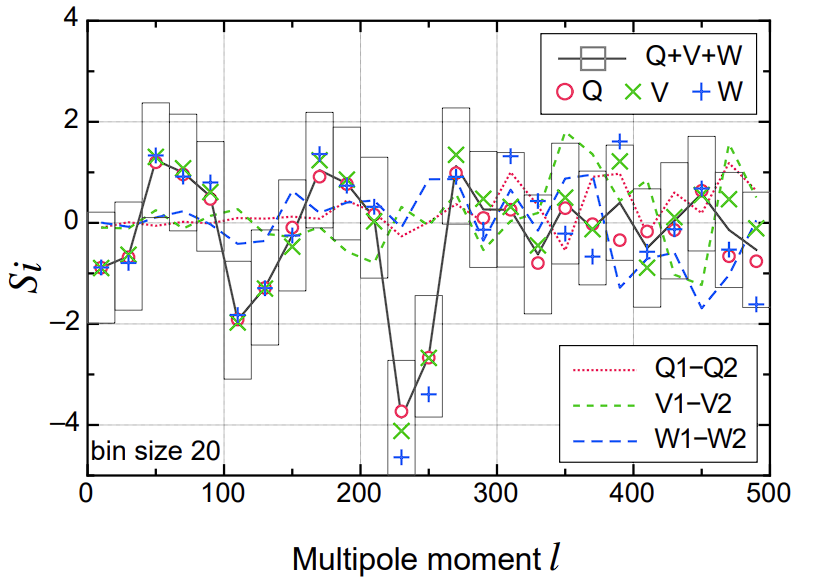
\includegraphics[width=0.8\linewidth]{DSE-Test Graph}
    \caption{The decorrelated band mean spectrum obtained by the seven-year WMAP data. The boxes and solid line are the result of the overall combined map (Q+V+W) and color data points are the results of the individual frequency maps (Q, V, W). The horizontal width of boxes indicates the bin size $\Delta \ell = 20$ for calculating the binned mean spectrum. Image source: \cite{Kashino_2012}}
    \label{fig:Decorrelated Statistical Spectrum}
\end{figure}
\\
We should note that Figure \ref{fig:Decorrelated Statistical Spectrum} contains a bin of size 20. The bin size in this context refers to the range of multipole moments $\ell$ that are grouped together when calculating the test statistic $S_i$. Or, in other words, instead of analyzing each individual $\ell$ separately, we sum over a range of values (a bin).
Moreover, Figure \ref{fig:Decorrelated Statistical Spectrum} presents the plots for: \begin{itemize}
    \item $Q+V+W$: A combined dataset that merges all three frequency bands to improve the signal-to-noise ratio.
    \item $Q1-Q2, V1-V2, W1-W2$: These are difference maps, created by subtracting different detector readings of the same frequency band. Due to this, they primarily contain instrumental noise, since the real CMB signal cancels out when differencing measurements from the same frequency.
\end{itemize}
These maps help verify whether anomalies seen in the main dataset are truly cosmological or just instrumental artifacts.

Now, to understand this graph, note that:
$S_i > 0$ represents more temperature fluctuations than expected at that scale.
Therefore, $S_i < 0$ corresponds to fewer temperature fluctuations than expected on that scale. In short, larger absolute values of $S_i$ correspond to a stronger deviation from isotropy. 
Moreover, to understand the multipole moment $\ell$ and what it represents in the graph, we can break it down into three main scenarios: 

\begin{itemize}
  \item Deviations only at high $\ell$ (small scales, $\ell > 300$): This would correspond to deviations caused by instrumental noise or foreground contamination \cite{Kashino_2012}.
  
  \item Deviations only at low $\ell$ (large scales, $\ell < 50$): This would correspond to deviations caused by large-scale anisotropies, potentially challenging the assumption of a statistically isotropic universe \cite{Bielewicz_2004}\cite{Pedro_2013}.

  \item Deviations on both large and small scales: This could indicate a more fundamental cosmological effect affecting multiple scales.
\end{itemize}

In Figure \ref{fig:Decorrelated Statistical Spectrum} we can see that the most significant anomaly appears in the mid-range multipoles ($221 \leq \ell \leq 240$), where $S_i$ is strongly negative, suggesting that the mean spherical harmonic coefficients at this scale are lower than expected compared to a statistically isotropic model. In other words, this means that temperature fluctuations at these angular scales are weaker than predicted by standard cosmological models. 
Thus, we can say that these results suggest something unexpected at these angular scales. But what is the cause? we can take a look at the three main scenarios stated above for the multipole moment $\ell$ ranges.
In our graph, we account for instrumental noise with the plots for $Q1-Q2, V1-V2, W1-W2$. Since the anomalies appear in $Q+V+W$ but not in $Q1-Q2$, $V1-V2$, or $W1-W2$, it suggests they are not due to noise, but instead a real cosmic effect. Moreover, the significant anomaly occurs at $221 \leq \ell \leq 240$, not at high $\ell$ ($\ell > 300$), where the noise-dominated behavior appears. This means that instrumental noise alone cannot explain the observed anomaly.\
Similarly, the strongest deviation we observe is at intermediate scales $221 \leq \ell \leq 240$, not at very large scales ($\ell < 50$). Thus, our anomaly does not directly suggest a large-scale anisotropy.
If we try to look at deviations at both large and small scales simultaneously. In this case, the main anomaly is localized in a particular range of $\ell$, rather than appearing at both low and high $\ell$. So, this suggests that it is not a fundamental cosmological effect affecting multiple scales.

The presence of an anomaly at $221 \leq \ell \leq 240$ suggests a possible connection to models of a finite curved universe. In a positively curved space (e.g., a three-sphere), allowed wave modes are quantized, which could lead to certain multipoles scales being preferred or suppressed in the CMB power spectrum.
The results of this article, although not conclusive, support the idea that the universe (or at least the CMB sky) has a small preferred direction. Supporting the idea of a non-trivial topology in the universe, specifically a spherical one. Which is analyzed more into detail in the other articles discussed in the other sections. 
As a final note, the analysis is limited by the existing data for the CMB temperatures. Thus, future high-resolution independent CMB observations like PLANCK will further refine these methods, offering deeper insights into the fundamental nature of the universe and the topology of space-time.



\section{Conclusion}

\begin{figure}[H]
    \centering
    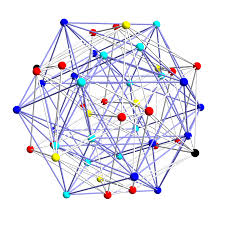
\includegraphics[width=0.25\linewidth]{binary-octahedron.png}
    \caption{
In conclusion, the universe has a strange shape, and everything you knew is a lie. Fear the binary octahedral, for the end is near.}
    \label{fig:binary-octahedron}
\end{figure}

We have designed and outlined a study of CMB temperature fluctuations in spherical spaces. We introduced spherical 3-manifolds as a plausible class of cosmological models and developed the mathematical tools (topology and eigenmode analysis) to handle them. Using these tools, we describe how one can compute CMB anisotropy patterns for a given spherical topology. We then connected these predictions to real data, discussing how one would recognize the fingerprint of a closed spherical universe in CMB observations ( such as through statistical anisotropies). Our synthesis of results from the articles by Aurich et al., Kashino et al., Pranav et al., and others shows that while no specific spherical topology is confirmed, the concept remains consistent with current data and even offers potential explanations for certain anomalies. It is relevant to mention that ongoing refinements in both theory and measurement could yet reveal a topological signature.
%\printbibliography

%apalike-ejor IAS THE 

\bibliographystyle{plain}
\bibliography{sources.bib}



\end{document}

